% Copyright 2004 by Till Tantau <tantau@users.sourceforge.net>.
%
% In principle, this file can be redistributed and/or modified under
% the terms of the GNU Public License, version 2.
%
% However, this file is supposed to be a template to be modified
% for your own needs. For this reason, if you use this file as a
% template and not specifically distribute it as part of a another
% package/program, I grant the extra permission to freely copy and
% modify this file as you see fit and even to delete this copyright
% notice.

\documentclass{beamer}

\usepackage[utf8]{inputenc}
\usepackage[portuguese]{babel}

% There are many different themes available for Beamer. A comprehensive
% list with examples is given here:
% http://deic.uab.es/~iblanes/beamer_gallery/index_by_theme.html
% You can uncomment the themes below if you would like to use a different
% one:
%\usetheme{AnnArbor}
%\usetheme{Antibes}
%\usetheme{Bergen}
%\usetheme{Berkeley}
%\usetheme{Berlin}
%\usetheme{Boadilla}
%\usetheme{boxes}
%\usetheme{CambridgeUS}
%\usetheme{Copenhagen}
%\usetheme{Darmstadt}
\usetheme{Dresden}     % Legal!
%\usetheme{default}
%\usetheme{Frankfurt}
%\usetheme{Goettingen}
%\usetheme{Hannover}
%\usetheme{Ilmenau}
%\usetheme{JuanLesPins}
%\usetheme{Luebeck}
%\usetheme{Madrid}
%\usetheme{Malmoe}
%\usetheme{Marburg}
%\usetheme{Montpellier}
%\usetheme{PaloAlto}
%\usetheme{Pittsburgh}
%\usetheme{Rochester}
%\usetheme{Singapore}
%\usetheme{Szeged}      % Legal!
%\usetheme{Warsaw}

%\usecolortheme{default}
\usecolortheme{rose}

% Include pagination (might not work for other themes)
\expandafter\def\expandafter\insertshorttitle\expandafter{%
   \insertshorttitle\hfill\insertframenumber\,/\,\inserttotalframenumber}

\newcommand{\quotes}[1]{``#1''}

% Hide navigation controls
\beamertemplatenavigationsymbolsempty

\title{Análise do uso de \textit{feedback} de relevância no Sistema de Integração Lattes-Qualis (SILQ)}

% A subtitle is optional and this may be deleted
% \subtitle{Optional Subtitle}

\author{Carlos Bonetti\inst{1}}
% - Give the names in the same order as the appear in the paper.
% - Use the \inst{?} command only if the authors have different
%   affiliation.

\institute[Universidade Federal de Santa Catarina] % (optional, but mostly needed)
{
  \inst{1}%
  Bacharelando de Ciência da Computação\\
  Departamento de Informática e Estatística\\
  Centro Tecnológico\\
  Universidade Federal de Santa Catarina\\
  \hfill \\
  Orientação: Profª. Drª. Carina F. Dorneles
  %\and
  %\inst{2}%
  %Department of Theoretical Philosophy\\
  %University of Elsewhere
}
% - Use the \inst command only if there are several affiliations.
% - Keep it simple, no one is interested in your street address.

\date{Trabalho de Conclusão de Curso, 2016/2}
% - Either use conference name or its abbreviation.
% - Not really informative to the audience, more for people (including
%   yourself) who are reading the slides online

% \subject{Theoretical Computer Science}
% This is only inserted into the PDF information catalog. Can be left
% out.

% If you have a file called "university-logo-filename.xxx", where xxx
% is a graphic format that can be processed by latex or pdflatex,
% resp., then you can add a logo as follows:

% \pgfdeclareimage[height=0.5cm]{university-logo}{university-logo-filename}
% \logo{\pgfuseimage{university-logo}}

% Delete this, if you do not want the table of contents to pop up at
% the beginning of each subsection:
%\AtBeginSubsection[]
%\AtBeginSection[]
%{
%  \begin{frame}<beamer>{Sumário}
    %\tableofcontents[currentsection,currentsubsection]
%    \tableofcontents[currentsection]
%  \end{frame}
%}

% ===========================================================================
% Let's get started

\begin{document}

\begin{frame}
  \titlepage
\end{frame}

%\begin{frame}{Sumário}
%  \tableofcontents
%  % You might wish to add the option [pausesections]
%\end{frame}

\section{Introdução}

\subsection{Histórico e Justificativa}

\begin{frame}{Lattes}
  \begin{figure}
    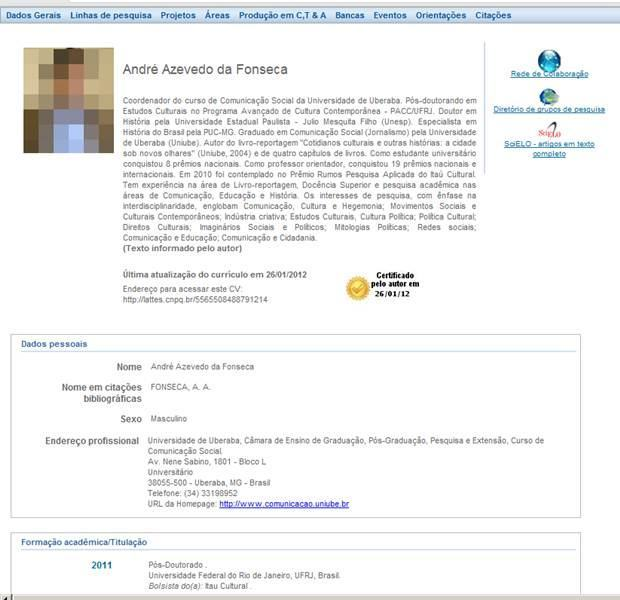
\includegraphics[scale=0.3]{figuras/lattes.jpg}
  \end{figure}
\end{frame}

\begin{frame}{Qualis}
  \begin{figure}
    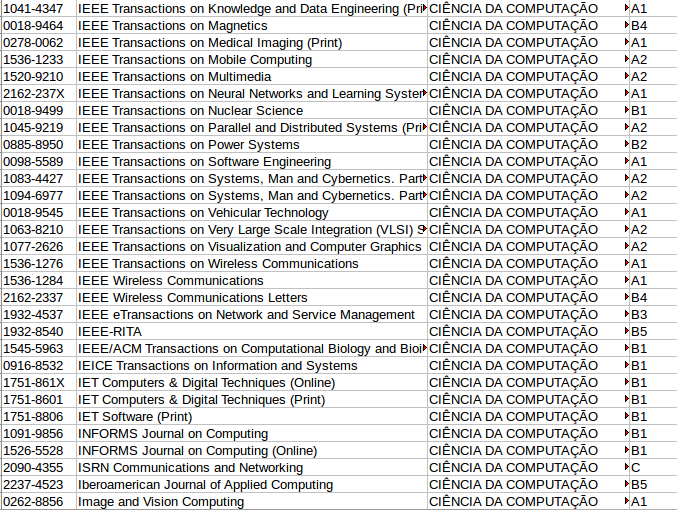
\includegraphics[scale=0.4]{figuras/qualis_exemplo.png}
  \end{figure}
\end{frame}

\begin{frame}{Histórico e Justificativa}
  \begin{itemize}
    \item AGUIAR, Felipe Nedel de; COSTA, Maria Eloísa. \textbf{SILQ - Sistema de Integração Lattes Qualis}. Trabalho de Conclusão de Curso. Florianópolis: Universidade Federal de Santa Catarina, Biblioteca Universitária, 2015.
    \item Qualificação automática de produções científicas através de busca por similaridade textual nos dados Qualis;
  \end{itemize}
\end{frame}

\begin{frame}
  \begin{figure}
    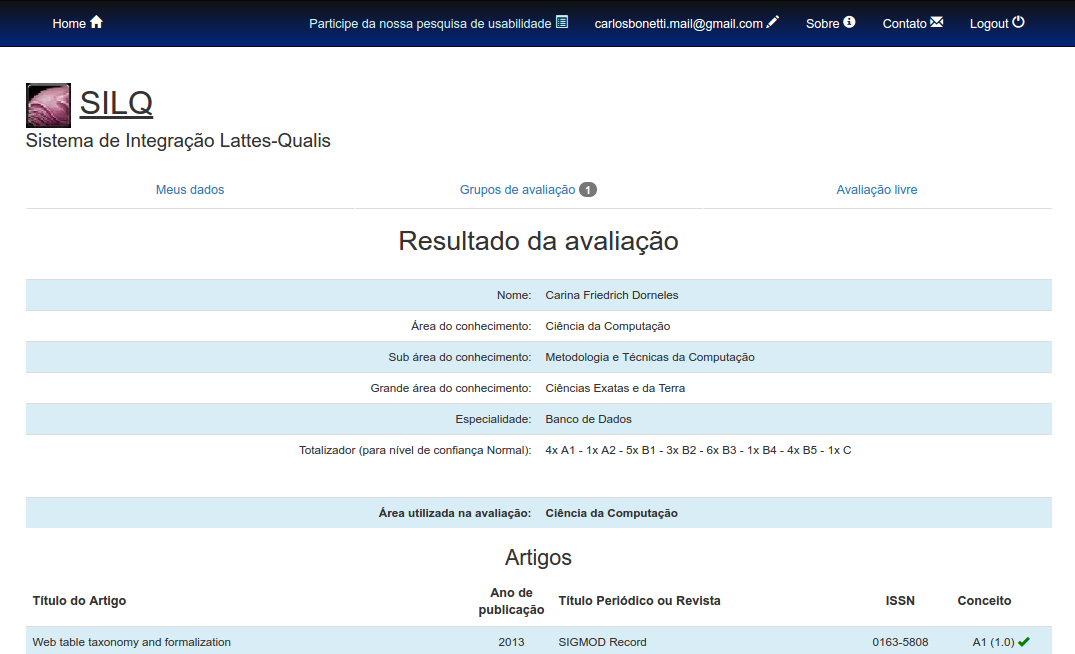
\includegraphics[width=\textwidth]{figuras/silq1-3.png}
    \caption{Primeira versão do SILQ (\url{http://silq.inf.ufsc.br})}
  \end{figure}
\end{frame}

\subsection{Como funciona o SILQ 1}

\begin{frame}{IR e Data Matching}
  \begin{itemize}
    \item \textit{Information Retrieval} (IR)
    \begin{itemize}
      \item \textit{query}
      \item documentos
    \end{itemize}

    \item \textit{Data-Matching}
    \begin{itemize}
      \item similaridade / dissimilaridade
      \item \textit{threshold}
    \end{itemize}
  \end{itemize}
\end{frame}

\begin{frame}{\textit{n-grams} / \textit{trigrams}}
  \quotes{Revista}: $ A = \{\_\_R,\_Re,Rev,evi,vis,ist,sta,ta\_\}$ \\
  \quotes{Revisor}: $ B = \{\_\_R,\_Re,Rev,evi,vis,iso,sor,or\_\}$ \\

  \hfill \\
  5 elementos em comum: $|A \cap B|$\\
  11 elementos distintos: $|A \cup B|$\\

  \hfill \\
  $
  \texttt{trigrams(Revista, Revisão)} = {|A \cap B| \over |A \cup B|} = {5 \over 11} = 0.45 = 45\%
  $
\end{frame}

\begin{frame}{Como o SILQ avalia um currículo Lattes}
  \underline{Trabalho \#1} (extraído do Lattes)\\
  \textbf{Título}: A Strategy for Allowing Meaningful and Comparable Scores in Approximate Matching\\
  \textbf{Ano}: 2007\\
  \textbf{Área}: Ciência da Computação\\
  \textbf{Evento}: Conference on Information and Knowledge Management (CIKM)\\

  \pause
  \hfill \\
  query: (título do evento, área)\\
  $q_T$ = (\texttt{Conference on Information and Knowledge Management (CIKM)}, \texttt{Ciência da Computação})
\end{frame}

\begin{frame}
  $q_T$ = (\texttt{Conference on Information and Knowledge Management (CIKM)}, \texttt{Ciência da Computação})

  \pause
  \footnotesize
  \begin{table}
    \begin{tabular}{ c | c | p{6.5cm} }
      \textbf{Conceito} & \textbf{Similaridade} & \textbf{Título}\\
      \hline \hline

      A1 & 0.71 & International Conference on Information and Knowledge Management\\ \hline
      B4 & 0.64 & International Conference on Information, Process, and Knowledge Management\\
    \end{tabular}
    \caption{Resultados retornados pelo SILQ para a query $q_T$}
  \end{table}

  \pause
  \normalsize
  \textbf{Resultado}\\
  Trabalho \#1 recebe o conceito A1
\end{frame}

\begin{frame}
  \begin{itemize}
    \item SILQ: sistema de IR baseado em \textit{data matching}
    \item Utiliza \texttt{trigrams} para \textit{matching} entre eventos informados no Lattes e os registrados no Qualis
    \item \textit{Threshold} de 0.6 (`nível de confiança normal')
  \end{itemize}
\end{frame}

\section{Objetivos}
\subsection*{Objetivos}

\begin{frame}{Motivação}
  \begin{itemize}
    \item Atualização tecnológica e da base de dados
    \begin{itemize}
      \item Qualis trienal $\rightarrow$ anual
      \item Atualização da base de dados Qualis no SILQ
      \item Considerar ano na \textit{query}
    \end{itemize}

    \item Qual o \textit{threshold} ideal para o SILQ?
    \item Qual a taxa de acerto do sistema? Ele está avaliando corretamente os currículos Lattes?
    \item É possível aumentar a taxa de acerto utilizando \textit{feedback} de usuários?
  \end{itemize}
\end{frame}

\begin{frame}{Objetivos}
  \begin{block}{Objetivo geral}
    Analisar o impacto que o uso de feedback de relevância tem na precisão dos resultados de avaliações realizadas pelo SILQ, efetuado sobre uma nova arquitetura da ferramenta que inclui a criação de API de integração com outros sistemas e a atualização da base de dados conforme as novas classificações Qualis.
  \end{block}
\end{frame}

\begin{frame}{Objetivos específicos}
  \begin{enumerate}
    \item<1-> Reestruturação da arquitetura e banco de dados do SILQ a fim de suportar classificações de eventos e periódicos disponibilizados em um ritmo anual;

    \item<1-> Atualização do banco de dados do sistema com as últimas classificações disponibilizadas pelo Qualis (anos 2013 e 2014);

    \item<2-> Criação de uma API pública de disponibilização dos serviços do SILQ, via camada de aplicação REST para integração com outros sistemas;
  \end{enumerate}
\end{frame}

\begin{frame}{Objetivos específicos}
  \begin{enumerate}[<+->]
    \setcounter{enumi}{3}

    \item Alterações na interface do sistema incluindo migração de \textit{framework} de interface, inclusão de controles de \textit{feedback}, novos gráficos de acompanhamento de grupos de pesquisa e melhorias gerais de usabilidade;

    \item Propor novos algoritmos de avaliação baseados em similaridade textual e \textit{feedback} de relevância e verificar se a taxa de acerto do sistema foi melhorada com tal ação.
  \end{enumerate}
\end{frame}

\section{Conceitos}
\subsection*{Conceitos}

\begin{frame}{\textit{Feedback} de relevância}
  \begin{itemize}
    \item Característica de sistemas IR
    \item Utilização de dados do usuário para melhorar sua precisão
    \item Explícito / Implícito
  \end{itemize}
\end{frame}

\begin{frame}{Métricas e avaliação de sistemas de IR}
  \begin{itemize}
    \item Como saber se o sistema retorna os resultados corretos?
    \item Avaliação baseado em métricas
    \item Taxa de acerto (\textit{accuracy} / exatidão*)
  \end{itemize}
\end{frame}

\section{Desenvolvimento}

\subsection{Alterações tecnológicas}

\begin{frame}{Extração e inserção dos novos dados Qualis}
  \begin{itemize}
    \item Até final de 2015
    \begin{itemize}
      \item Qualis trienal
      \item 2010-2012
      \item PDFs e planilhas XLS
    \end{itemize}

    \item Início de 2016
      \begin{itemize}
        \item Qualis anual
        \item 2010, 2011, 2012, 2013, 2014
        \item Planilhas CSV
      \end{itemize}

    \item Limpeza manual (erros de codificação, ISSNs omitidos, etc.)
    \item 339.204 registros
  \end{itemize}
\end{frame}

\begin{frame}{Atualização tecnológica}
  \begin{itemize}
    \item Criação da camada REST de integração
    \begin{itemize}
      \item API pública de acesso aos dados Qualis e serviços do SILQ
    \end{itemize}
    \item Migração de \textit{framework}: \textit{Play} $\rightarrow$ \textit{Spring}
    \item Reescrita do \textit{front-end} com \textit{AngularJS}
    \begin{itemize}
      \item Novos gráficos de avaliação para grupos de pesquisa
      \item Melhorias no módulo de usuários
      \item Remodelagem da página de resultados de avaliação
      \item Inclusão dos controles de \textit{feedback}
    \end{itemize}
    \item Garantida da qualidade com testes automatizados
  \end{itemize}
\end{frame}

\begin{frame}
  \begin{figure}
    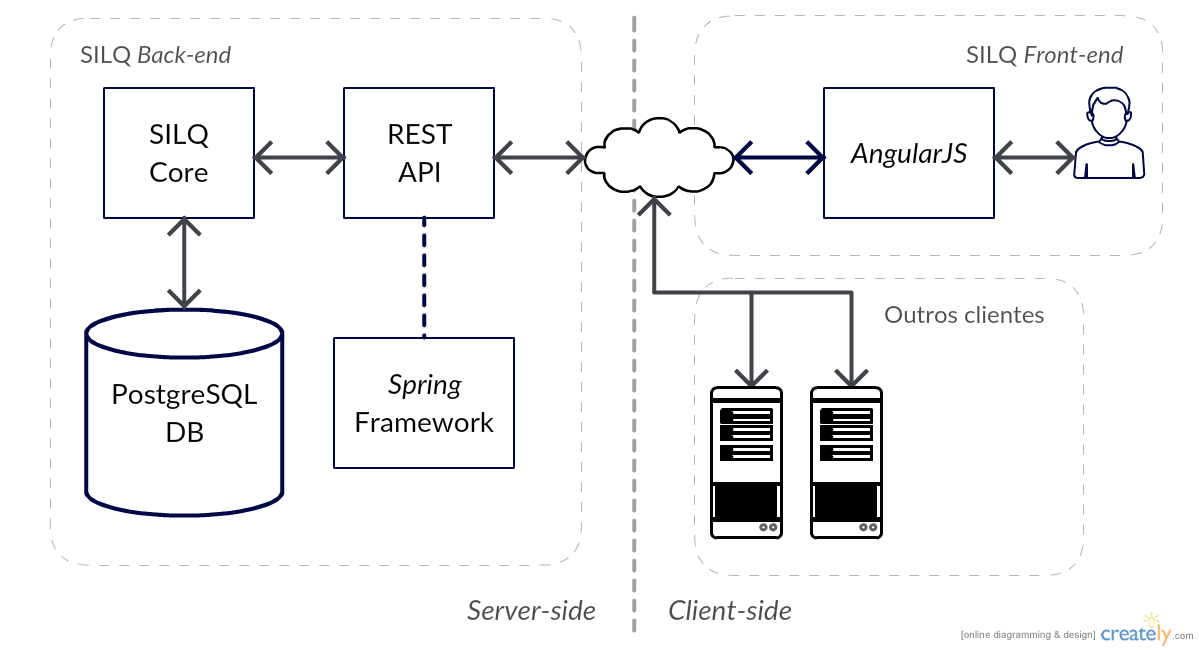
\includegraphics[width=\textwidth]{figuras/arquitetura-silq.png}
    \caption{Nova arquitetura do SILQ}
  \end{figure}
\end{frame}

\begin{frame}
  \begin{figure}
    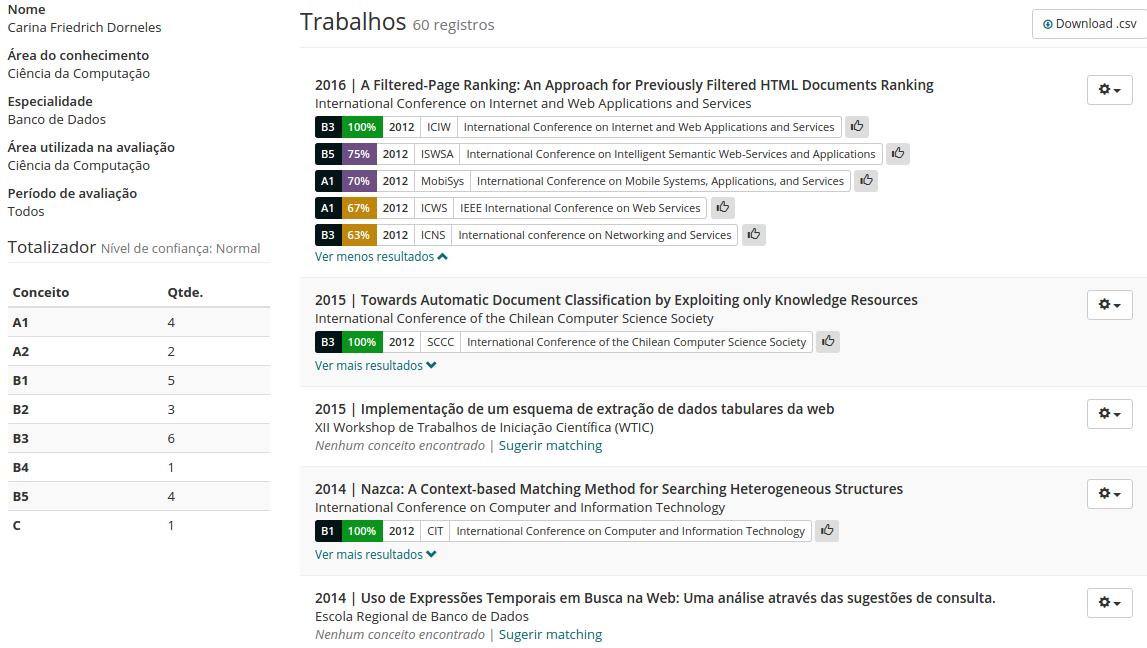
\includegraphics[width=\textwidth]{figuras/avaliacao-silq2.png}
    \caption{Nova página de avaliação do SILQ}
  \end{figure}
\end{frame}

\subsection{Uso de feedback de relevância}

\begin{frame}{Obtenção de feedback}
  \begin{figure}
    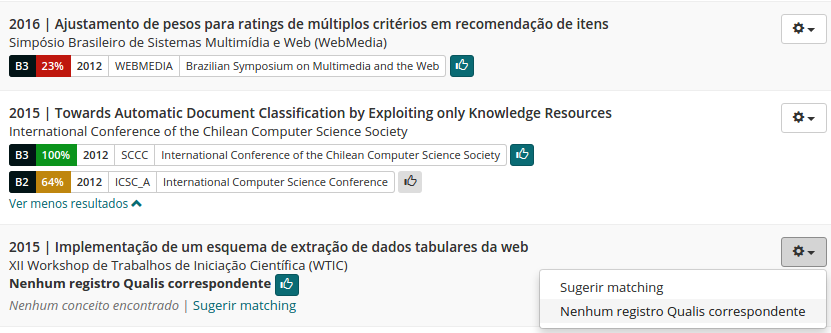
\includegraphics[width=\textwidth]{figuras/feedbacks.png}
    \caption{Controles de feedback da página de resultados de avaliação do SILQ}
  \end{figure}
\end{frame}

\begin{frame}{Algoritmos}
  \begin{itemize}
    \item De que forma utilizar o \textit{feedback} obtido?
    \item Criação de algoritmos baseados no \textit{trigrams} do SILQ 1
    \begin{itemize}
      \item \texttt{fb(t)}
      \item \texttt{query\_aliasing}
    \end{itemize}
    \item Avaliação experimental
  \end{itemize}
\end{frame}

\begin{frame}{Algoritmo \texttt{fb(1)}}
  $q_1$ = (\quotes{Software Engineering Knowledge Engineering}, 2009, CCO)\\

  \pause
  \small
  \begin{table}[!h]
    \begin{tabular}{ c | p{7cm} | c }
      \textbf{\#} & \textbf{Evento} & \textbf{Similaridade} \\ \hline
      \hline

      1 & Software Engineering and Data Engineering (SEDE) & 0.53 \\ \hline
      2 & International Conference on Software Engineering and Knowledge Engineering (SEKE) & 0.49 \\ \hline
      ... & ... & ...
    \end{tabular}
  \end{table}

  \pause
  \textbf{feedback 1:} (ID Qualis, \textit{query})\\
  $f_1$ = (\#2, \quotes{Software Engineering Knowledge Engineering})
\end{frame}

\begin{frame}{Algoritmo \texttt{fb(1)}}
  \framebox[\textwidth][l]{
    \small
    $f_1$ = (\#2, \quotes{Software Engineering Knowledge Engineering})
  }

  \hfill \\
  $q_2$ = (\quotes{Software Engineering Knowledge Engineering}, 2010, CCO)\\

  \pause
  \small
  \begin{table}[!h]
    \begin{tabular}{ c | p{7cm} | c }
      \textbf{\#} & \textbf{Evento} & \textbf{Similaridade} \\ \hline
      \hline

      2 & International Conference on Software Engineering and Knowledge Engineering (SEKE) & 0.49 \\ \hline
      1 & Software Engineering and Data Engineering (SEDE) & 0.53 \\ \hline
      ... & ... & ...
    \end{tabular}
  \end{table}

  $f_1$ utilizado, \textit{match} realizado com evento \#2
\end{frame}

\begin{frame}{Algoritmo \texttt{fb(1)}}
  \begin{enumerate}
    \item Cria o \textit{rank} inicial de resultados utilizando a função \texttt{trigrams} (idêntico ao SILQ 1)
    \item Pesquisa por \textit{feedback} anterior \underline{idêntico} à \textit{query} submetida
    \item Caso exista, adiciona o Qualis atribuído ao \textit{feedback} na primeira posição do \textit{rank}
  \end{enumerate}
\end{frame}

\begin{frame}{Algoritmo \texttt{fb(1)}}
  \framebox[\textwidth][l]{
    \small
    $f_1$ = (\#2, \quotes{Software Engineering Knowledge Engineering})
  }

  \hfill \\
  $q_3$ = (\quotes{Software Engineering \textbf{and} Knowledge Engineering}, 2011, CCO)\\

  \pause
  \begin{itemize}
    \item Feedback 1 não é considerado
    \item \texttt{fb(1)} considera somente \textit{queries} \underline{idênticas}
    \item \texttt{fb(t)}: Considerar também \textit{feedbacks} com \textit{queries} \underline{similares}!
    \begin{itemize}
      \item $t$: \textit{threshold} de similaridade de \textit{feedback}
    \end{itemize}
  \end{itemize}
\end{frame}

\begin{frame}{Algoritmo \texttt{fb(t)}}
  \framebox[\textwidth][l]{
    \small
    $f_1$ = (\#2, \quotes{Software Engineering Knowledge Engineering})
  }

  \hfill \\
  $q_3$ = (\quotes{Software Engineering \textbf{and} Knowledge Engineering}, 2011, CCO)\\

  Similaridade: 0.88 (\textit{trigrams})\\
  \pause
  Considerando \textit{fb(0.75)}:\\

  \small
  \begin{table}[!h]
    \begin{tabular}{ c | p{7cm} | c }
      \textbf{\#} & \textbf{Evento} & \textbf{Similaridade} \\ \hline
      \hline

      2 & International Conference on Software Engineering and Knowledge Engineering (SEKE) & 0.49 \\ \hline
      1 & Software Engineering and Data Engineering (SEDE) & 0.53 \\ \hline
      ... & ... & ...
    \end{tabular}
  \end{table}
\end{frame}

\begin{frame}{Algoritmo \texttt{fb(t)}}
  \begin{enumerate}
    \item Cria o \textit{rank} inicial de resultados utilizando a função \texttt{trigrams} (idêntico ao SILQ 1)
    \item Pesquisa pelo \textit{feedback} anterior mais \underline{similar} à \textit{query} submetida e cuja similaridade seja $t$ ou superior
    \item Caso exista, adiciona o Qualis atribuído ao \textit{feedback} na primeira posição do \textit{rank}
  \end{enumerate}
\end{frame}

\begin{frame}{Algoritmo \texttt{fb(t)}}
  \begin{itemize}
    \item Qual o valor de $t$ ideal?
    \item Desconsidera os valores de similaridade do \textit{rank} inicial
    \item \textit{Rank} não é mais ordenado por similaridade
  \end{itemize}
\end{frame}

\begin{frame}{Algoritmo \texttt{query\_aliasing}}
  \framebox[\textwidth][l]{
    \small
    $f_1$ = (\#2, \quotes{Software Engineering Knowledge Engineering})
  }

  \hfill \\
  $q_4$ = (\quotes{Software Engineering \textbf{and} Knowledge Engineering}, 2011, CCO)\\

  Similaridade: 0.88 (\textit{trigrams})\\

  \pause
  \small
  \begin{table}[!h]
    \begin{tabular}{ c | p{7cm} | c }
      \textbf{\#} & \textbf{Evento} & \textbf{Rank} \\ \hline
      \hline

      2 & International Conference on Software Engineering and Knowledge Engineering (SEKE) & \textbf{0.88} \\ \hline
      1 & Software Engineering and Data Engineering (SEDE) & 0.53 \\ \hline
      ... & ... & ...
    \end{tabular}
  \end{table}
\end{frame}

\begin{frame}{Algoritmo \texttt{query\_aliasing}}
  \begin{enumerate}
    \item Cria o \textit{rank} inicial de resultados utilizando a função \texttt{trigrams} (idêntico ao SILQ 1)
    \item Pesquisa pelo \textit{feedback} anterior mais \underline{similar} à \textit{query} submetida
    \item Caso exista, adiciona o Qualis atribuído ao \textit{feedback} na lista de resultados com valor de \textit{rank} igual ao valor de similaridade entre a nova \textit{query} e a \textit{query} do \textit{feedback}
  \end{enumerate}
\end{frame}

\begin{frame}{Avaliação experimental}
  \begin{itemize}
    \item Conjunto de testes
    \begin{itemize}
      \item 33 currículos de pesquisadores do PPGCC
      \item 300 trabalhos aleatoriamente selecionados e avaliados manualmente
    \end{itemize}

    \item Comparação entre o resultado retornado pelo sistema e o resultado selecionado
  \end{itemize}
\end{frame}

\begin{frame}{Avaliação de \textit{threshold} ideal}
  \begin{figure}
    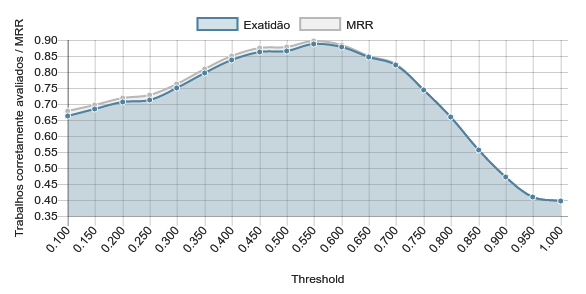
\includegraphics[width=\textwidth]{figuras/avaliacao-threshold.png}
    \caption{Valores de exatidão e MRR para diferentes valores de \textit{threshold} utilizando o método \textit{trigram}}
  \end{figure}
\end{frame}

\begin{frame}{Exatidão dos algoritmos propostos}
  \begin{table}
    \begin{tabular}{ c | c }
      \textbf{Algoritmo} & \textbf{Exatidão} \\
      \hline \hline
      \textit{trgm} & 88.667\% \\
      \textit{trgm + fb(1.00)} & 89.667\% \\
      \textit{trgm + fb(0.90)} & 90.667\% \\
      \textit{trgm + fb(0.80)} & 92.667\% \\
      \textit{trgm + fb(0.70)} & 92.667\% \\
      \textit{trgm + fb(0.60)} & 91.000\% \\
      \textit{trgm + query\_aliasing} & \textbf{93.333}\%
    \end{tabular}
    \caption{Comparação da exatidão dos diferentes algoritmos testados (utilizando \textit{threshold} de $0.55$)}
  \end{table}
\end{frame}

\begin{frame}
  \begin{figure}
    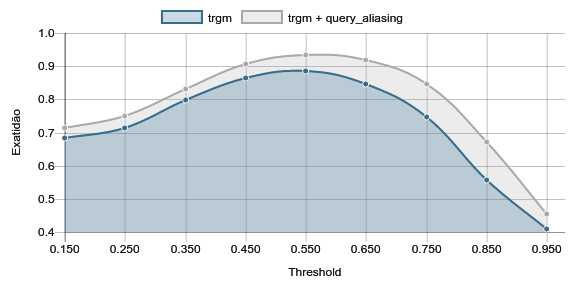
\includegraphics[width=\textwidth]{figuras/avaliacao-algoritmos.png}
    \caption{Comparação da taxa de acerto do algoritmo \textit{trgm} e do \textit{trgm + query\_aliasing} para diferentes \textit{thresholds}}
  \end{figure}
\end{frame}

\section{Conclusões}
\subsection*{Conclusões}

\begin{frame}{Conclusões}
  \begin{itemize}[<+->]
    \item Criação da camada REST de integração
    \begin{itemize}[<1->]
      \item Ex.: \url{http://silq.inf.ufsc.br/api/qualis}
    \end{itemize}
    \item Atualização da base de dados com os novos registros Qualis
    \item Métricas de exatidão do sistema
    \item Descoberto \textit{threshold} ideal: 0.55
    \item Inserção dos controles de \textit{feedback} de relevância
    \item Taxa de acerto média do sistema melhorada de 87\% para 93.3\% com o uso de \textit{feedback} de usuários e \texttt{query\_aliasing}
    \item SILQ 2: \url{http://silq.inf.ufsc.br}
  \end{itemize}
\end{frame}

\begin{frame}{Trabalhos futuros}
  \begin{itemize}[<+->]
    \item Avaliar outras funções de similaridade
    \item Avaliar diferentes estratégias de uso de \textit{feedback} de relevância
    \begin{itemize}[<1->]
      \item Ex.: Algoritmo de Rocchio, \textit{machine learning}, etc
    \end{itemize}
    \item Tradução de nomes de eventos
    \item Automatizar ainda mais o processo de avaliação de Programas de Pós-Graduação conforme regras da CAPES
    \begin{itemize}[<1->]
      \item Gerar valores de $I_{geral}$ e $I_{restrito}$
      \item Utilizar pesos considerados pela CAPES
    \end{itemize}
  \end{itemize}
\end{frame}

\appendix
\section<presentation>*{\appendixname}
\subsection<presentation>*{Encerramento}

\begin{frame}
  \begin{center}
    \large {\usebeamercolor[fg]{structure} Análise do uso de \textit{feedback} de relevância no Sistema de Integração Lattes-Qualis (SILQ)}

    \hfill \break

    \LARGE Obrigado!

    \hfill \break
    \normalsize Carlos Bonetti \\
    \textit{carlosbonetti.mail@gmail.com}
  \end{center}
\end{frame}

\end{document}
